
\section{Part A}
\label{s:task1-part-a}
The file \lstinline{ImageFile7.001} will be the subject of the following report
as specified in the task document. All the steps shown in this report are to
guarantee that veracious and accurate procedures are followed to safeguard the
preservation of the evidence and are suitable to be served in court. To
establish evidence, stages are documented and explained.

\subsection{Correct Image}
\label{s:task1-part-a-correct-image}
As a demonstration that the image file is the correct one, verification has been
carried out. The following dialog represents the MD5 Hash that confirms it is an
exact copy of the original file.

\begin{figure}[H]
  \centering
  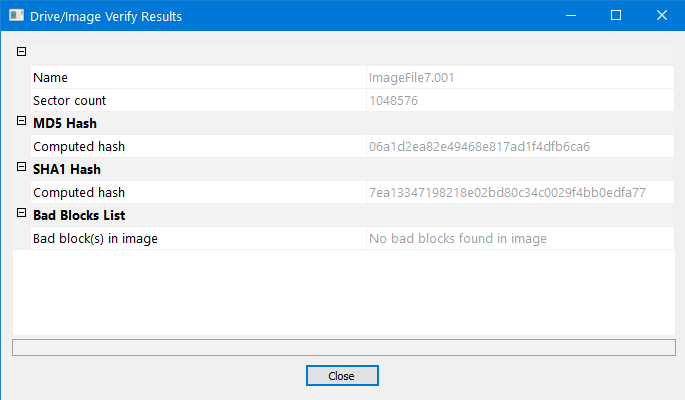
\includegraphics[width=0.7\textwidth]{figures/hash}
  \caption{Image Hash}
  \label{f:image-hash}
\end{figure}

\subsection{EWF/E01 Image Files}
\label{s:task1-part-a-ewf-e01-file}
For this tasks, two different methods and images are being created. To create
the images, the dialog to create images has been opened on \lstinline{FTK Imager}.

\begin{figure}[H]
  \centering
  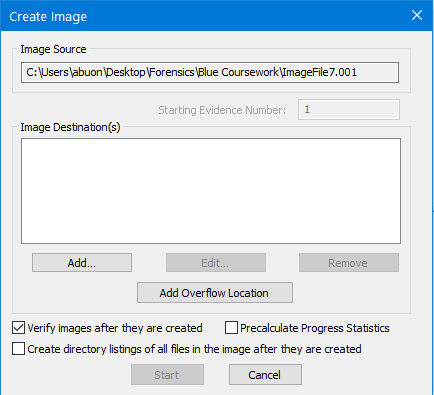
\includegraphics[width=0.6\textwidth]{figures/create-images}
  \caption{Create Images on FTK Imager}
  \label{f:create-images}
\end{figure}

Clicking on \lstinline{Add} will open another dialog that asks for evidence
information.

\begin{figure}[H]
  \centering
  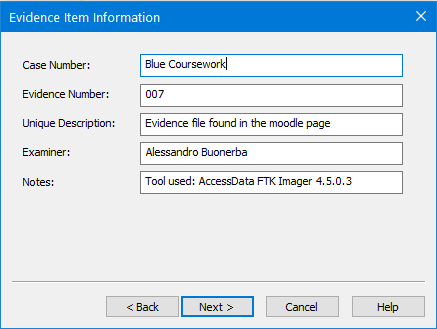
\includegraphics[width=0.6\textwidth]{figures/evidence-information}
  \caption{Evidence Information}
  \label{f:evidence-information}
\end{figure}

The next step is used to selected the image destination, the filename and
various options such as fragmentation and compression.

\begin{figure}[H]
  \centering
  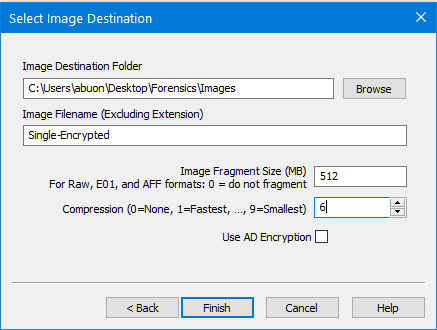
\includegraphics[width=0.6\textwidth]{figures/single-encrypted}
  \caption{Single Encrypted Image}
  \label{f:single-encrypted}
\end{figure}

The figure above represents the first requirements that asks to create a single
E01 image file with enabled compression that in this case is set on 6, while the
figure below represents the splitted version without compression.

\begin{figure}[H]
  \centering
  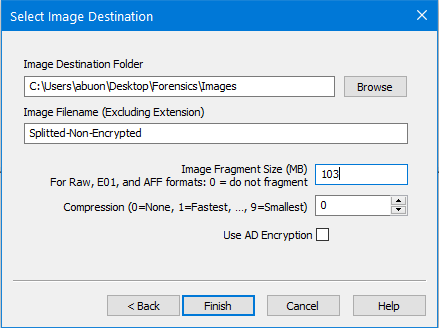
\includegraphics[width=0.6\textwidth]{figures/splitted-no-compression}
  \caption{Fragmented Image without Compression}
  \label{f:splitted-no-compression}
\end{figure}

Since the image to be split is 512mb and the new E01 must be split in 5 files,
the image fragment size has been set dividing the two numbers, resulting in
103mb. After closing the dialog, the previous create image dialog is shown again
with the image destinations and configurations that has been set previously for
the two tasks.

\begin{figure}[H]
  \centering
  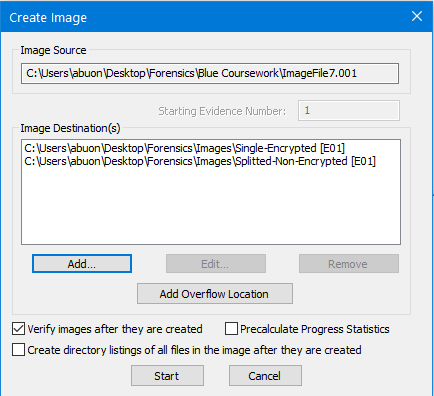
\includegraphics[width=0.6\textwidth]{figures/create-image-start}
  \caption{Create Image Dialog with Images}
  \label{f:create-image-start}
\end{figure}

Clicking on start will initialise the creation of both and at the end of the
process a verify result dialog will pop up with informations on both image
output and their hashes.

\begin{figure}[H]
  \centering
  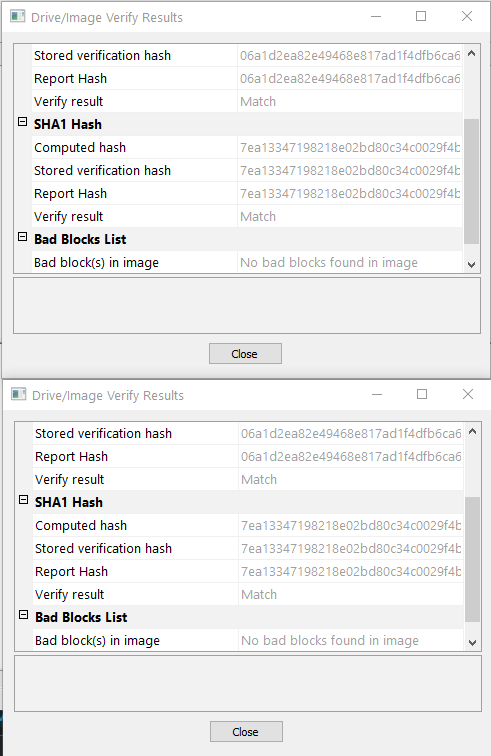
\includegraphics[width=0.5\textwidth]{figures/end-process-hashes}
  \caption{Verify Result Dialog}
  \label{f:end-process-hashes}
\end{figure}

The following image captures the structure of the output files we previously
created. It confirms that the splitted files are indeed 5.

\begin{figure}[H]
  \centering
  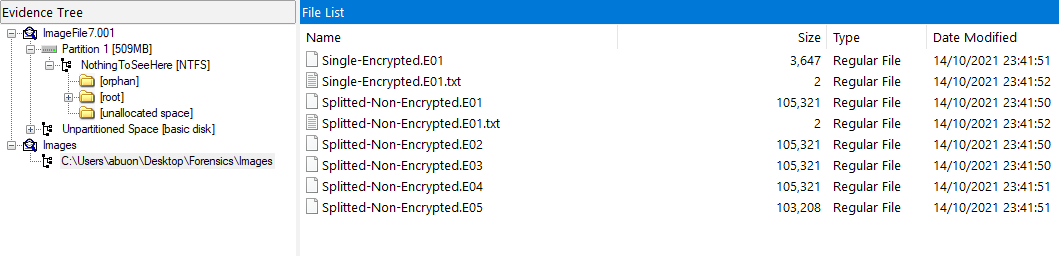
\includegraphics[width=0.8\textwidth]{figures/folder-structure}
  \caption{File Structures}
  \label{f:folder-structure}
\end{figure}

\section{Part B}
\label{s:task1-part-b}
Previously, \lstinline{FTK Imager} has been used to accomplish the tasks, and
the previously screenshots to document the hashes of the images created. To
perform Dual Tool Verification, \lstinline{Autopsy} is also used on this task to
double-check the image hashes. The following screenshots confirm that the hashes
are the same, meaning that nothing has been tempered.

\begin{figure}[H]
  \centering
  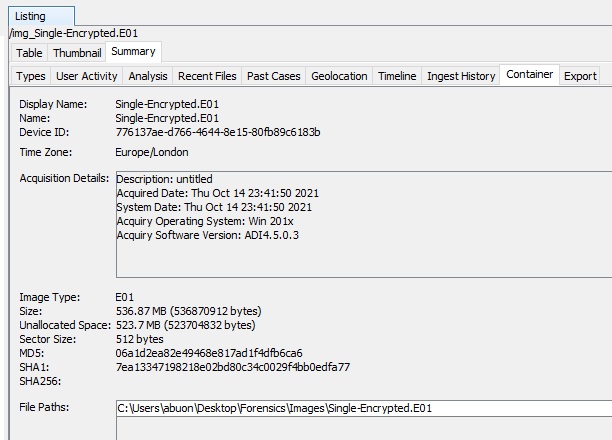
\includegraphics[width=0.7\textwidth]{figures/autopsy-hashes}
  \caption{Autopsy Dual Tool Verification}
  \label{f:autopsy-hashes}
\end{figure}

\newpage
\section{Part C}
\label{s:task1-part-c}
The following would be a description suitable for the members of a jury without
technical knowledge.

\subsection{Write blocker}
\label{s:write-blocker}
A \lstinline{Write blocker} is a small portable device used by investigators to examine USBs
or other removable media without tempering the evidences that are being examined,
preserving authenticity.
